%%%%%%%%%%%%%%%%%%%%%%%%%%%%%%%%%%%%%%%%%%%%%%%%%%%%%%%%%%%%%%%%%%%%%%%%%%%%%%%%
%2345678901234567890123456789012345678901234567890123456789012345678901234567890
%        1         2         3         4         5         6         7         8

\documentclass[letterpaper, 10 pt, conference]{ieeeconf}  % Comment this line out
                                                          % if you need a4paper
%\documentclass[a4paper, 10pt, conference]{ieeeconf}      % Use this line for a4
                                                          % paper

\IEEEoverridecommandlockouts                              % This command is only
                                                          % needed if you want to
                                                          % use the \thanks command
\overrideIEEEmargins
% See the \addtolength command later in the file to balance the column lengths
% on the last page of the document

\usepackage[utf8]{inputenc}
\usepackage[T1]{fontenc}
\usepackage{graphicx}
\usepackage{textgreek}
\usepackage{xcolor}
\usepackage{tabularx}
\usepackage{makecell}


% The following packages can be found on http:\\www.ctan.org
%\usepackage{graphics} % for pdf, bitmapped graphics files
%\usepackage{epsfig} % for postscript graphics files
%\usepackage{mathptmx} % assumes new font selection scheme installed
%\usepackage{mathptmx} % assumes new font selection scheme installed
%\usepackage{amsmath} % assumes amsmath package installed
%\usepackage{amssymb}  % assumes amsmath package installed

\title{\LARGE \bf
An Investigative Survey Into the Intersection of Consumer Trust and Password Security
}

%\author{ \parbox{3 in}{\centering Huibert Kwakernaak*
%         \thanks{*Use the $\backslash$thanks command to put information here}\\
%         Faculty of Electrical Engineering, Mathematics and Computer Science\\
%         University of Twente\\
%         7500 AE Enschede, The Netherlands\\
%         {\tt\small h.kwakernaak@autsubmit.com}}
%         \hspace*{ 0.5 in}
%         \parbox{3 in}{ \centering Pradeep Misra**
%         \thanks{**The footnote marks may be inserted manually}\\
%        Department of Electrical Engineering \\
%         Wright State University\\
%         Dayton, OH 45435, USA\\
%         {\tt\small pmisra@cs.wright.edu}}
%}

\author{David Kwan$^{1}$% <-this % stops a space
\thanks{$^{1}$D. Kwan is a Master's student in the School of Information Technology, Faculty of Liberal Arts \& Professional Studies, York University, 4700 Keele St, Toronto
        {\tt\small dkwan33@yorku.ca}}%
}


\begin{document}


\maketitle
\thispagestyle{empty}
\pagestyle{empty}


%%%%%%%%%%%%%%%%%%%%%%%%%%%%%%%%%%%%%%%%%%%%%%%%%%%%%%%%%%%%%%%%%%%%%%%%%%%%%%%%
\begin{abstract}

In this paper, I present a study into the intersection of password security and trust. Through the use of a survey, I explore the association between password strength, password security habits, consumer trust in various websites, and the impact of password security training, age, and education. I find that there is an association between password strength and password security training. I observe a lack of association between age or education with security factors. Furthermore I discuss the notion of consumer trust as it relates to password security and explore trends and methods of measurement.

\end{abstract}


%%%%%%%%%%%%%%%%%%%%%%%%%%%%%%%%%%%%%%%%%%%%%%%%%%%%%%%%%%%%%%%%%%%%%%%%%%%%%%%%
\section{Introduction and Literature Review}

Password security is an omnipresent consideration in our daily lives. We use passwords to protect our personal data everywhere, be it internet banking, e-commerce, social media, or any one of an uncountable number of websites that utilize personal accounts. 

We must first define what constitutes password security. Password security is not simply password strength, although that is certainly one of the two major aspects of it, security also includes the habits and actions we take that compromise security \cite{Dhamija2000}. Password strength itself is composed of both the length and complexity of the password \cite{Morris1979}. Certainly, longer passwords with a larger pool of possible characters are harder to crack via brute-force. The weaker the password, the easier it is to brute-force. However, for a stronger password, the probability that a brute-force attack will succeed decreases drastically \cite{DellAmico2010}.

Password strength meters are present during account creation on many websites. These meters certainly guide users to choose stronger passwords, but are not necessarily always present \cite{DeCarnavalet2014}. In the absence of an enforced password strength policy, people tend to choose weaker passwords \cite{DellAmico2010}. 

The habits that compromise our password security are re-use and writing-down \cite{Dhamija2000}. Our forgetfulness, or rather the memorability of our passwords, is a major factor that leads to both password re-use and writing them down. Brown et al. in their study on remembrance and memorability found that a majority of respondents re-use their passwords, and in fact, duplicate them identically \cite{Brown2004}. Password managers are software that auto-generate strong passwords and remember them for us. As long as the manager used is secure, then your passwords are fairly secure \cite{Alkaldi2016}. Unfortunately they are not that widely used. It is still much more common to custom-create your own password \cite{Alkaldi2016}.

Data breaches have been occurring over the last decade with alarming frequency. Some famous ones include dating website Ashley Madison’s breach in 2015, question-and-answer site Quora in 2018, and cryptocurrency wallet Gatehub in 2019. Password re-use, regardless of the website, enables hackers to access accounts on any websites with that shared password. Thomas et al. in 2017 found that 25\% of the passwords from data breaches matched the same user’s google account \cite{Thomas2017}. 

The occurrence of a data breach is not only a risk to our personal data, but it in fact lowers our trust in that website, company, or service \cite{Curtis2018}. When there hasn’t been a data breach (yet), however, our trust is closely linked to the perceived level of security of the website. We trust websites that appear more secure \cite{Flavian2006}.
Thusly, we arrive at the core questions of this paper: Do we use stronger passwords on certain websites related to our perceived level of trust in that website? I postulate that we do to some extent, for the sake of memorability. Do we have habits that weaken or strengthen our password security? Does our password security change based on whether we have had training on the matter? Our education level in general? Our age? 

Although there has been much research done on what is a strong password, behaviors that make for strong password security, and what influences consumer trust; there has been a lack of research that specifically targets the intersection of password strength and trust. Brown et al., in their discussions, suggested that if security needs are minimal then people should choose a common password that is easy to remember, and if security is essential then choose one that is cryptic \cite{Brown2004}. This paper aims to address, to some extent, all of these questions and investigate any possible relationships to stimulate more research and strengthen previous research.

\section{Hypotheses}

The following are the 9 pairs of null and alternate hypotheses tested. They were created after factor analysis to reduce the number of possible dimensions for statistical analysis. It is important to note here that the term “password strength with a consideration of trust” is a confusing notion. This is unintentional but unavoidable as the intent of this research is to explicitly test whether trust influences password security practice. We will use descriptive statistics to investigate this relationship, but inferential statistics could not be performed due to problems in research design and will be elaborated on in the discussion section.

\begin{itemize}
\item H\textsubscript{1o}: There is no difference in password strength between those who are trained and untrained in password security.
\item H\textsubscript{1a}: There is a difference in password strength between those who are trained and untrained in password security.
\item H\textsubscript{2o}: There is no difference in password strength with a consideration for consumer trust between those who are trained and untrained in password security.
\item H\textsubscript{2a}: There is a difference in password strength with a consideration for consumer trust between those who are trained and untrained in password security.
\item H\textsubscript{3o}: There is no difference in password security habits between those who are trained and untrained in password security.
\item H\textsubscript{3a}: There is a difference in password security habits between those who are trained and untrained in password security.
\item H\textsubscript{4o}: There is no difference in password strength between those who are above or below 44 years of age.
\item H\textsubscript{4a}: There is a difference in password strength between those who are above or below 44 years of age.
\item H\textsubscript{5o}: There is no difference in password strength with a consideration for consumer trust between those who are above or below 44 years of age.
\item H\textsubscript{5a}: There is a difference in password strength with a consideration for consumer trust between those who are above or below 44 years of age.
\item H\textsubscript{6o}: There is no difference in password security habits between those who are above or below 44 years of age.
\item H\textsubscript{6a}: There is a difference in password security habits between those who are above or below 44 years of age. 
\item H\textsubscript{7o}: There is no difference in password strength between those have graduate degrees and those who do not.
\item H\textsubscript{7a}: There is a difference in password strength between those have graduate degrees and those who do not.
\item H\textsubscript{8o}: There is no difference in password strength with a consideration for consumer trust between those have graduate degrees and those who do not.
\item H\textsubscript{8a}: There is a difference in password strength with a consideration for consumer trust between those have graduate degrees and those who do not.
\item H\textsubscript{9o}: There is no difference in password security habits between those have graduate degrees and those who do not.
\item H\textsubscript{9a}: There is a difference in password security habits between those have graduate degrees and those who do not.

\end{itemize}


\section{Research Design}

\subsection{Sampling and Instrumentation}

The research method used was a survey questionnaire. Sampling was nonrandom as the sample chosen was a convenience sample with the intent of maximizing the possible sample size. Four groups of participants were surveyed: the first being a class of Information Systems Master’s students at York University (including the professor), the second being a group of young professionals at a social gathering, the third being friends and family of the researcher, and the last being employees at a small business in the food industry. In total, 40 participants were surveyed. The participants were not told what exactly the intent of the research was, just that the survey is “about password strength”, although due to the wording of the questions on the survey, I surmise it was not particularly difficult to guess the intent of the survey.

The survey was administered in-person only rather than on-line or hybrid. Participants were verbally asked for consent, in addition to the written consent at the top of the first page of the survey. This in-person survey method minimizes the possibility of participants dropping out (e.g. disconnecting) in the middle of filling-out the questionnaire, as well as non-response issues. During the survey process, it was common for participants to not realize there were 2 pages to the questionnaire. However, since the survey process was done in-person, the researcher was able to remind participants to fill out both pages and, in the end, all 40 questionnaires were filled to completion. This survey method eliminates the possibility of participants submitting more than one questionnaire, as the researcher could personally keep track of who had already been given a questionnaire. An on-line or hybrid survey may have been beneficial to increase sample size, but would have resulted in validity concerns.

The questionnaire consisted of 15 questions (See Appendix A for a blank copy of the questionnaire). 3 of the questions were demographic questions, while the other 12 were criterion questions. The first 5 of these questions were measured on a 5-option Likert-like rating scale. The 7 questions were measured on a 5-option standard agree or disagree Likert scale.  The primary criterion questions regarding password strength are presented first, and the demographic questions were presented last to maximize reader interest and thus lower the possibility of nonresponse. A logical navigational path for the criterion questions was followed. In particular, questions 1 to questions 5 ask the reader to rate the strength of their passwords on various types of websites rather than spreading them around the survey.

Every question was analyzed for the possibility of being misleading (ie: loaded, leading, or double-barreled). Neutral language was used whenever possible, although, for the questions that are scored on agree or disagree Likert scales, there must still be a “direction” for the question that the participant can either agree or disagree with. For example, rather than “My passwords are weak”, or “My passwords are strong”, “I tend to use strong passwords” was chosen to make the question feel as neutral as possible while still maintaining a direction. This does pose an internal validity concern, which will be discussed in section \ref{sec:internalvalidity}.

Furthermore, the questions were designed so they would be applicable to all participants. It was unlikely that participants would want or need to answer “not applicable” to any questions except questions 1 to 5. For questions 1 to 5, participants were instructed to leave the question blank if it did not apply to them. This did not prove to be necessary as there were no questions left unanswered on any of the questionnaires.  

Each survey was manually scored by the researcher and then reviewed a second time to minimize the possibility of manual scoring errors. Methods to improve reliability such as split-half reliability were considered, but ultimately not used due to the potential decrease in an already small sample size.

\subsection{A Brief Note on Likert Scales}

In this paper all Likert scales used on a scale of “agree” to “disagree” are treated as nominal measurements. It is unfit to place an order on “agreeing” or “disagreeing” to a question, as all opinions are equally valid and are thus inherently unordered. In scientific practice, Likert scales are commonly treated as ordinal scales, and in some cases even interval scales; a common argument in favor of interval, that equidistant steps can be inferred if the scale is symmetric \cite{Norman2010}. The Likert-like scales from “weak” to “strong” used in questions 1 to 5 are treated as ordinal. It is reasonable to consider the scale ordinal since it is a direct rating from weak to strong where strong can be said to be higher than weak.

\subsection{Variables}

The 3 demographic questions on the questionnaire measured three independent variables: the age of the participant, their general level of education, and their specific level of education with regards to password security. The intent of the latter was to gauge whether the participant had been formally taught what makes a strong password. 

The 12 criterion questions, at a basic level, all measured password strength or at least habits related to password strength, but with different nuances. The questionnaire was designed with 2 groups of questions:

The first group consists of the questions that deal with password strength as it relates to trust. Trust was either implicitly or explicitly built as a consideration in the question. Questions 1 to 5 asked participants to rate their password strength in different types of websites, with the assumption that participants have different levels of trust in different types of websites. Question 6 was a more direct method of measuring password strength vs general trust, asking participants whether they have stronger passwords based on their perceived trust of a website. Since trust is directly influenced by the security level perceived by consumers, question 7, which asks participants whether they have strong passwords based on the perceived security level of a website, was designed as both a repeat of question 6 and also as a method of confirming the relationship found in \cite{Flavian2006}. The intent of all the questions in this group was to investigate the suggestion by Brown et al. \cite{Brown2004} discussed earlier, but the design of the questions was poor and the implications of this will be elaborated on in section \ref{sec:results}.

The second group consists of the questions that measure password strength without regards to trust. Question 11 asked this directly, asking participants simply whether they used strong passwords. Questions 8, 9, 10, and 12 all asked participants about their behavior or habits that are closely linked to password strength. These behaviors being respondents' password re-use, writing passwords down, forgetting passwords, and their usage of auto-generated passwords.

\section{Results and Discussion}\label{sec:results}

\subsection{Descriptive Statistics}

\begin{table*}[h]
\caption{Calculated descriptive statistics for all questions}
\label{tab:desc}
\begin{center}
\begin{tabular}{rrrrrrrrrrrrrrrr}
\hline
      & Q1  & Q2 & Q3  & Q4 & Q5 & Q6  & Q7  & Q8  & Q9  & Q10 & Q11 & Q12 & Q13 & Q14 & Q15 \\ \hline
Mode   & 3,4 & 4  & 3,4 & 3  & 3  & 4   & 4   & 5   & 4   & 1   & 4   & 5   & 2   & 2   & 2   \\ \hline
Median & 4   & 3  & 3   & 3  & 3  & N/A & N/A & N/A & N/A & N/A & N/A & N/A & N/A & N/A & N/A \\ \hline
Range  & 4   & 5  & 4   & 5  & 5  & N/A & N/A & N/A & N/A & N/A & N/A & N/A & N/A & N/A & N/A \\ \hline
\end{tabular}
\end{center}
\end{table*}

Table \ref{tab:desc} shows the calculated descriptive statistics for every question. Since we are dealing with mostly nominal variables, we can only calculate the mode for the responses to questions 6 to 15.  Two questions had two modes, which are shown separated with a comma. From the mode we can see that there is not much variation in the answers for password strength with regards to trust in different websites (question 1 to question 5). Further analysis of the descriptive measures on these questions will be discussed in section \ref{sec:trust}. We can see that the mode for question 11 is “agree”, indicating that most respondents generally consider themselves to have strong passwords. The mode for questions 8, 9, and 10 are “strongly agree” (“strongly disagree” for Q10, but it is an inversely related question), indicating that respondents tend to re-use, write-down, and forget their passwords; supporting the current literature \cite{Brown2004}. The mode for question 12 is “strongly agree”, indicating that respondents tend to prefer custom-creating passwords rather than auto-generated, which supports the previous findings by Alkaldi et al. \cite{Alkaldi2016}.

The mode for both question 6 and question 7 is “agree”, indicating that respondents tend to agree that they have stronger password security when on websites that are more trustworthy or have better security. This trend is interesting because it indicates that respondents may be more concerned over potential loss in the event of a data breach rather than having strong passwords to compensate for a lack of security, thus preventing a possible data breach in the first place. One would expect that respondents would “agree” to this question if they are more concerned with the former, and to “disagree” if they are more concerned with the latter.

The mode for all three demographic questions (Questions 13-15) indicate that respondents tended to be younger, with bachelor’s level education, and some password security training.

\subsection{Factor Analysis}

\begin{table}[h]
\caption{Component Matrix for non-rotated PCA}
\label{tab:compmatrix}
\begin{center}
\begin{tabular}{lrrr}
\hline
                & 1     & 2     & 3     \\ \hline
Q1\_PStr\_Bank  & .759  & -.159 & -.236 \\ \hline
Q2\_PStr\_Shop  & .662  & .095  & .235  \\ \hline
Q3\_PStr\_Work  & .741  & .079  & -.063 \\ \hline
Q4\_PStr\_SMed  & .652  & -.390 & .387  \\ \hline
Q5\_PStr\_Forum & .608  & -.370 & -.019 \\ \hline
Q6\_PStr\_Trust & .577  & .647  & .005  \\ \hline
Q7\_PStr\_Sec   & .634  & .603  & .115  \\ \hline
Q8\_PReuse      & -.560 & .244  & .301  \\ \hline
Q9\_PForget     & .071  & .325  & .784  \\ \hline
Q10\_PWrite     & .103  & .673  & -.269 \\ \hline
Q11\_PStr       & .714  & -.248 & -.298 \\ \hline
Q12\_PCustom    & -.173 & .329  & -.620 \\ \hline
\end{tabular}
\end{center}
\end{table}

\begin{table}[h]
\caption{Component Matrix for rotated PCA}
\label{tab:compmatrixrot}
\begin{center}
\begin{tabular}{lrrr}
\hline
                & 1     & 2     & 3     \\ \hline
Q1\_PStr\_Bank  & .759  & -.159 & -.236 \\ \hline
Q2\_PStr\_Shop  & .662  & .095  & .235  \\ \hline
Q3\_PStr\_Work  & .741  & .079  & -.063 \\ \hline
Q4\_PStr\_SMed  & .652  & -.390 & .387  \\ \hline
Q5\_PStr\_Forum & .608  & -.370 & -.019 \\ \hline
Q6\_PStr\_Trust & .577  & .647  & .005  \\ \hline
Q7\_PStr\_Sec   & .634  & .603  & .115  \\ \hline
Q8\_PReuse      & -.560 & .244  & .301  \\ \hline
Q9\_PForget     & .071  & .325  & .784  \\ \hline
Q10\_PWrite     & .103  & .673  & -.269 \\ \hline
Q11\_PStr       & .714  & -.248 & -.298 \\ \hline
Q12\_PCustom    & -.173 & .329  & -.620 \\ \hline
\end{tabular}
\end{center}
\end{table}

\begin{figure}[thpb]
  \centering
%   \framebox{\parbox{3in}{
    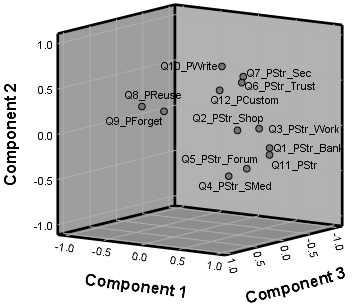
\includegraphics[scale=0.84]{compplot1.PNG}
% }}
  \caption{Non-rotated Component Plot}
  \label{fig:compplot}
\end{figure}
  
\begin{figure}[thpb]
  \centering
%   \framebox{\parbox{3in}{
    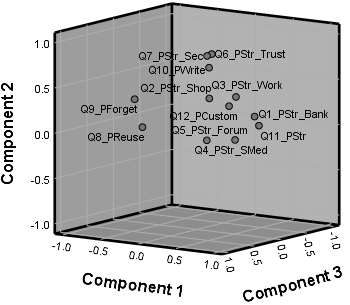
\includegraphics[scale=0.84]{compplotrot.PNG}
% }}
  \caption{Rotated Component Plot}
  \label{fig:compplotrot}
\end{figure}

Factor analysis was performed on the 12 criterion variables to determine which variables were highly correlated. Factor analysis allows us to reduce the number of dimensions on which the criterion variables can be compared with demographic variables. Factor analysis was performed via Principal Component Analysis (PCA), and was initially not rotated. The results of PCA showed that there were 3 components. The question of which variable belonged to which component was not initially clear from the 3-dimensional component plot (Fig. \ref{fig:compplot}), and so PCA was performed a second time using Varimax Rotation with Kaiser Normalization for robustness and to ease the identification of component variables. The resulting 3-dimensional component plot (Fig. \ref{fig:compplotrot}) in rotated space did not give substantially more readable components. In-fact, Question 12 appears to be more closely correlated to component 1 than component 2 in rotated space, but from the component matrices we can see that this is not the case. 

\subsection{Component Composition and Representation}

From the component matrices and the component plots, it can be determined that the components are as follows:

\begin{enumerate}
\item 	Component 1 consists of questions 1-5, and 11.
\item 	Component 2 consists of questions 6, 7, 10, and 12.
\item 	Component 3 consists of questions 8 and 9.
\end{enumerate}

These components were surprising, and the components here are reasonable in some cases, and a little perplexing in others. First, I will discuss the most reasonable representations of each component. 

Component 1 represents password strength, and I surmise that it is password strength with no consideration for consumer trust. Question 11, which directly asked the participant to rate their password strength is most highly correlated with this component. Questions 1 to 5 are all also highly correlated, indicating questions 1 to questions 5 may be simply directly related to password strength and had no real effect on measuring password strength as it relates to trust. For the purposes of statistical analysis with the demographic variables, question 11 will be used since it is most highly correlated with the component.

Component 2 likely represents password strength with a consideration for consumer trust. Question 6 and Question 7, which directly ask participants to rate their password strength with regards to consumer trust are the most highly correlated variables to the factor. Question 10, which asked whether participants write down their passwords, is also highly correlated. This, at least at an initial glance, is perplexing. One would think that writing down passwords would be inversely correlated to password strength. Upon further analysis however, this positive correlation with password strength may make sense since people are more likely to write down their passwords if their password is complex or long. From this point of view, the positive correlation is reasonable. Question 12 is also a perplexing relationship. Question 12 asked whether or not participants use their own passwords rather than auto-generated passwords. Using your own passwords, while not necessarily being stronger than auto-generated passwords, may give the illusion that the password is strong from a psychological perspective. It is surprising that questions 1 to 5 are not highly correlated with this factor, since they were designed to be more specific forms of question 6 and question 7. For the purposes of statistical analysis with the demographic variables, question 6 will be used since it is most highly correlated with the component.

Component 3 represents variables that measure habits or practices that result in poor password security. Question 9, regarding password forgetfulness is most highly correlated with this factor and is likely to represent this factor, since there are only two members anyway. Furthermore, I am hesitant to include question 8 in this component, since on the component matrices it has a weak correlation to component 3, and is, in fact, mathematically more strongly correlated in an inverse relationship to component 1. From a logical standpoint, it could reasonably belong in either one. Question 8 essentially asks participants to rate their level of password re-use. Password re-use could be positively correlated with component 3, since high forgetfulness indicates high password re-use. On the other hand, low password re-use also indicates high password security. For the purposes of statistical analysis with the demographic variables, question 9 will be used since it is most highly correlated with the component.

%   \begin{figure}[thpb]
%       \centering
%       \framebox{\parbox{3in}{We suggest that you use a text box to insert a graphic (which is ideally a 300 dpi TIFF or EPS file, with all fonts embedded) because, in an document, this method is somewhat more stable than directly inserting a picture.
% }}
%       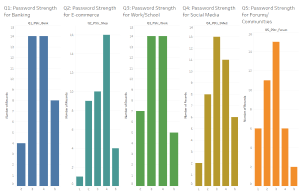
\includegraphics[scale=1.0]{barsQ1Q5300w.PNG}
%       \caption{Inductance of oscillation winding on amorphous
%       magnetic core versus DC bias magnetic field}
%       \label{fig:barchartsmall}
%   \end{figure}
   
% Figure Labels: Use 8 point Times New Roman for Figure labels. Use words rather than symbols or abbreviations when writing Figure axis labels to avoid confusing the reader. As an example, write the quantity ``Magnetization'', or ``Magnetization, M'', not just ``M''. If including units in the label, present them within parentheses. Do not label axes only with units. In the example, write ``Magnetization (A/m)'' or ``Magnetization {A[m(1)]}'', not just ``A/m''. Do not label axes with a ratio of quantities and units. For example, write ``Temperature (K)'', not ``Temperature/K.''

\subsection{Hypotheses From Factor Analysis}

Before performing any statistical analysis, the demographic results for each of questions 13 to 15 were grouped into 2 groups each. Question 13: password security training, was divided into “some or less” and “more than some”. Question 14: age, was divided into below 44 and above 44 years of age. Question 15: education level, was divided into those who have graduate degrees and those who do not. These groupings were created so that more powerful 2-sample statistical tests could be performed on the demographic variables. Phi correlation testing was also performed on the ungrouped demographic variables for investigative purposes.

Using each representative of each component, we can test the statistical difference between the components and each grouped demographic variable, resulting in 9 pairs of null and alternate hypotheses seen in section 1.1.

\subsection{Analysis Between Components and Demographic Variables}

Since all of the 15 variables collected, as well as the 3 transformed (grouped) variables, are measured on a nominal or ordinal scale, then all variable results must be nonparametric. The tests used were Fisher’s exact test to determine if there were nonrandom associations between the 2-sample grouped demographic variables and our criterion components. The Chi-Square test was not available in place of Fisher’s exact test because the sample size did not allow for the 5-minimum count in every cell. In every case at least one cell had less than 5 samples. Kruskal-Wallis tests could not be performed because the test requires the dependent variable to be at least measured on an ordinal scale. Measures of correlation were also performed using Cramer’s V. Since it is more important to investigate the entire breadth of the demographic variables, the ungrouped variables were used for correlational tests. The ungrouped variables are not dichotomous decisions, thus Cramer’s V, commonly called Cramer’s Phi was used in place of the Phi Coefficient. 

For all statistical testing, a critical value of \textalpha{}=0.05 was used. The traditional alternative of \textalpha{}=0.01 was not chosen. This way, the possibility of type 2 errors was minimized so as not to miss capturing any correlation or relationship between the variables. 

Two-tailed tests were performed rather than one-tailed tests because the research problem makes no assumptions on the direction of any relationships. Only to investigate whether that relationship exists. For example we cannot suppose whether younger or older people have better password security.

\begin{table}[h]
\caption{Fisher's exact test p-values for grouped demographics vs component representatives}
\label{tab:fisher}
\begin{center}
\begin{tabular}{lrrr}
\hline
                & Q13 GROUP & Q14 GROUP & Q15 GROUP \\ \hline
Q11 Component 1 & \textcolor{red}{0.010}       & 0.736       & 0.193       \\ \hline
Q6 Component 2  & 0.526       & 0.732       & 0.305       \\ \hline
Q9 Component 3  & 0.977       & 0.358       & 0.688       \\ \hline
\end{tabular}
\end{center}
\end{table}

Table \ref{tab:fisher} shows the resulting p-values from Fisher’s exact test performed on all pairings of the 2-sample grouped demographic variables with the component representatives. In total all 9 possible pairings are shown. The only pairing where p < \textalpha{} is between Q11 vs Q13 marked in red. Recall that Q11 directly asked for password strength, while question 13 measured their level of password security training. We can reject H\textsubscript{1o} and accept H\textsubscript{1a}. Thus, there exists a statistically significant difference between those with “some or less” password security training and those with “more than some” password security training. This finding is reasonable, as you would expect those who have been trained in password security to have better knowledge and practice of password strength. All other null hypotheses are accepted.

\begin{table}[h]
\caption{Cramer’s V for correlational tests between ungrouped demographics and component representatives}
\label{tab:cramer}
\begin{center}
\begin{tabular}{lrrr}
\hline
                & Q13   & Q14   & Q15   \\ \hline
Q11 Component 1 & 0.395 & 0.336 & 0.307 \\ \hline
Q6 Component 2  & 0.346 & 0.282 & 0.396 \\ \hline
Q9 Component 3  & 0.220 & 0.344 & 0.326 \\ \hline
\end{tabular}
\end{center}
\end{table}

\begin{table}[h]
\caption{P-values for correlational tests between ungrouped demographics and component representatives.}
\label{tab:cramerp}
\begin{center}
\begin{tabular}{lrrr}
\hline
                & Q13   & Q14   & Q15   \\ \hline
Q11 Component 1 & 0.096 & 0.319 & 0.503 \\ \hline
Q6 Component 2  & 0.277 & 0.691 & 0.093 \\ \hline
Q9 Component 3  & 0.924 & 0.273 & 0.386 \\ \hline
\end{tabular}
\end{center}
\end{table}

Table \ref{tab:cramer} shows the resulting Cramer’s V values for correlation tests performed on all pairings of the ungrouped demographic variables with the component representatives. At a glance we can see all the pairings are positively correlated, but the correlations are relatively weak. Table \ref{tab:cramerp} shows the corresponding p-values for each pairing, and we can see p > \textalpha{} in all cases and thus none of the pairings reach significance threshold.

\subsection{Trust, Password Security, and Issues Therein}\label{sec:trust}

  \begin{figure*}[thpb]
  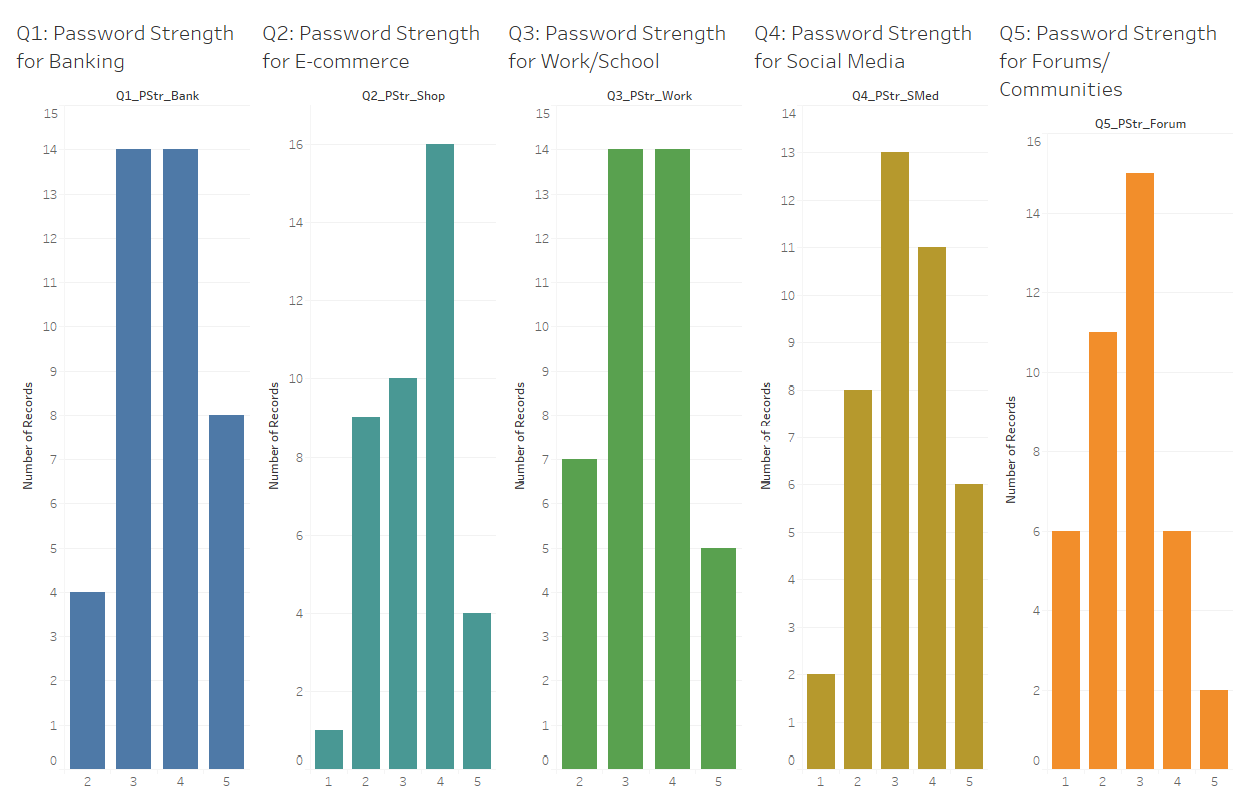
\includegraphics[width=1.0\textwidth]{barsQ1Q5.PNG}
     \caption{Distribution of answers by strength rating for trust-category questions}
         \label{fig:barchart}
  \end{figure*}

Fig. \ref{fig:barchart} shows the actual number of responses for each of questions 1 to 5 for each strength rating. Bars with 0 responses are not shown for conciseness. From an observational standpoint, we can see no immediate difference. Question 5 appears to have generally lower responses than the other 4 questions, but not by much. If we refer to Table \ref{tab:desc} and compare the modes, we can see that all the modes are either 3 or 4 with no discernable pattern. The medians are slightly more informative, but not by much. We can see that responses to all questions have a median of 3, except for banking passwords which have a median of 4. These observed trends are not trustworthy due to many threats to the internal validity of this study.

The goal of questions 1 to 5 was to investigate the relationship between various levels of trust in websites and the level of password strength used by participants. Admittedly, the instrumentation was poorly designed and could not effectively investigate this relationship in any meaningful fashion. The questions were designed in such a way that a scale of trust was inherently built into the questions from 1 to 5, with question 1, the question regarding banking passwords assumed to have the highest trust, and question 5, the question regarding internet communities assumed to have the lowest trust. The intent was to analyze differences between the answers to each question, but this design has several issues. Not only does this make an assumption that is not necessarily substantiated, but even between the questions the scale of trust is unclear. For example, it is unreasonable to say that one has more trust in social media websites vs e-commerce websites. 

Furthermore, because these are dependent variables with non-binary decisions, only the correlation between the variables could be statistically tested. Cramer’s V values were generated between the 5 variables for these 5 questions, and all 5 questions had high positive correlation; which confirms the results of factor analysis since they were all part of the same component. The high correlation indicates that regardless of website, stronger passwords beget stronger passwords. I have not shown the table of values because the problem with testing correlation is that it is not, in fact, a question we are interested in. It is reasonable and possibly obvious that password strength in one category of websites would be highly and positively correlated with password strength in another category. After all, one who has strong passwords in general would have strong passwords across all websites. We are not interested in the correlation between password strengths on different websites, but rather a significant difference between the means (which can only be calculated for continuous data). If there was a difference, then we would have been able to see if respondents use different password strengths for different categories of websites.

\subsection{Possible Changes for Further Research}

The core issue underlying why questions 1 to 5 were ineffective is that we lack concrete data on trust. Preferably continuous data, but at the very least ordinal data. Admittedly, continuous data on the notion of trust may be impossible, or at least extremely difficult to measure. Not only is making the assumption on levels of trust in different categories unfounded, but it has no frame of reference to compare with. There are many ways that this relationship could have been investigated in a much more robust and meaningful fashion, and I offer two suggestions here for both future work and the possibility of re-doing this study. Both methods would first require participants to rate their trust in various websites on an ordinal scale; this way there would be usable data on trust rather than an assumption.

\begin{enumerate}
\item The first method would then ask participants to rate their password strength on a similar scale in the same website. Then this variable could be directly checked for correlation with the trust variable.
\item The second method would instead ask participants to “check all websites” that they have strong password for. Each website would be treated during data coding as a binary choice and then these binary choices could be statistically compared to the trust rating. 
\end{enumerate}

\section{Research Validity}
\subsection{Threats to Internal Validity}\label{sec:internalvalidity}

There are many threats to internal validity of this study. Firstly, no reliability methods were used in questionnaire design. It is highly possible that there are respondents who could have answered inconsistently or even untruthfully. Usage of survey methods such as split-half or test-retest reliability design would have minimized this threat. 

Secondly, another instrumentation issue, the order of questions 1 to 5 may have indicated to the participants the answer that the survey “wanted”. It is reasonable to think that the order of the questions indicated a downwards hierarchy, and it is further reasonable to think that participants may have perceived this hierarchy. If the questionnaire was designed using method 1 from the previous section, and the question order was then randomized, then this threat could have been mitigated.

Thirdly, there is still a distinct possibility that the language used on some questions was not “neutral enough” and was slightly leading. Asking participants whether they have a “strong password” or agree with having “strong passwords” may have yielded different results than if the questionnaire asked for “weak password”. This threat may have been mitigated by sticking to either perfectly-neutral scales such as “please rate from 1-5” or by asking both strong and weak on the same questionnaire.

Lastly, the conditions under which the questionnaire was administered was not standardized. In the case of the graduate students, the condition was a classroom scenario where all participants were motivated to answer truthfully and completely, since not doing so would have been a social faux-pas. In the case of the young professionals, the conditions were loud and distracting. In the case of the friends and family, as well as the employees of a small company, the conditions were calm but the participants did not particularly incentivized to complete the questionnaire. Standardization, or at least some control, over the conditions would have aided in combatting this threat. Incentivization through the provision of a token would also have been beneficial.

\subsection{Threats to External Validity}\label{sec:externalvalidity}

There are many threats to the external validity of this study. Firstly, the sample size of the survey is both small and nonrandom. It is not reasonable to infer that this sample represents the true population. Since most of the respondents are post-secondary educated, and in the field of information technology no less, the results for password strength could be skewed on the high-end. This threat could have been mitigated with random sampling methods and a much larger sample size.

Secondly, the survey questionnaire is entirely subjective to what the respondent considers a “strong” password, and what the respondent considers “trustworthy” or “secure”. What the respondent considers a strong password may not be truly strong. Likewise, a website that a respondent considers trustworthy (or secure) may be different from how trustworthy that website is generally perceived. This is furthermore likely to be different from the actual security of the website, as perception and reality can be very different. It is unlikely a questionnaire could combat this threat effectively without revealing the respondent’s passwords, which would in turn be unethical. 

\section{Conclusion}

In this work I presented an investigative survey into password strength and password habits as they intersect with consumer trust, as well as their relationships with training, age, and education. I identified that there indeed exists an association between password strength and password security training. My work corroborates previous findings by Brown et al. \cite{Brown2004} on the prevalence of poor password security habits, as well as work by Alkaldi \& Renaud \cite{Alkaldi2016} on the unpopularity of password managers and auto-generated passwords. My work also illustrates the need for future work in this domain to be mindful of instrumentation for the measurement of trust, and the importance of further investigation into the notion of trust and how it affects our security.

% A conclusion section is not required. Although a conclusion may review the main points of the paper, do not replicate the abstract as the conclusion. A conclusion might elaborate on the importance of the work or suggest applications and extensions. Referring figure 2 = Fig. \ref{fig:barchart}. Let's cite c2 = \cite{c2}. 



%%%%%%%%%%%%%%%%%%%%%%%%%%%%%%%%%%%%%%%%%%%%%%%%%%%%%%%%%%%%%%%%%%%%%%%%%%%%%%%%



%%%%%%%%%%%%%%%%%%%%%%%%%%%%%%%%%%%%%%%%%%%%%%%%%%%%%%%%%%%%%%%%%%%%%%%%%%%%%%%%



%%%%%%%%%%%%%%%%%%%%%%%%%%%%%%%%%%%%%%%%%%%%%%%%%%%%%%%%%%%%%%%%%%%%%%%%%%%%%%%%
\section*{Appendix A: Questionnaire}
% Appendixes should appear before the acknowledgment.

This is a research survey created for studies at York University. Your participation in this survey is voluntary. The purpose of the research survey is to evaluate your trust in websites and the companies running those websites as well as your password creation and security practices. This survey should take you about 3 minutes to complete.

The survey will not ask you for your personal information or your passwords. The surveys will be kept \textbf{strictly confidential} and the questionnaires are \textbf{strictly anonymous}. All data will be aggregated prior to analysis and will only be used for the present study. The questionnaires will be destroyed after the publication of the results. If you have any questions, or would like a summary of the finds from this survey, please contact me at dkwan33@yorku.ca.

\textbf{Please Circle One Answer:}

\begin{enumerate}
    \item How would you rate the strength of the password(s) you use for your personal banking? \textit{Answer if applicable (e.g. TD Bank, RBC, Scotiabank)}
        \begin{table}[!htbp]
        \begin{center}
        \begin{tabular}{ccccc}
        1                 & 2        & 3       & 4     & 5              \\
        Very Weak & Weak & Average & Strong & Very Strong
        \end{tabular}
        \end{center}
        \end{table}
    \item How would you rate the strength of the password(s) you use for online shopping? \textit{Answer if applicable (e.g. Amazon, BestBuy, Loblaws)}
        \begin{table}[!htbp]
        \begin{center}
        \begin{tabular}{ccccc}
        1                 & 2        & 3       & 4     & 5              \\
        Very Weak & Weak & Average & Strong & Very Strong
        \end{tabular}
        \end{center}
        \end{table}
    \item How would you rate the strength of the password(s) you use for your work or school? \textit{Answer if applicable}
        \begin{table}[!htbp]
        \begin{center}
        \begin{tabular}{ccccc}
        1                 & 2        & 3       & 4     & 5              \\
        Very Weak & Weak & Average & Strong & Very Strong
        \end{tabular}
        \end{center}
        \end{table}
    \item How would you rate the strength of the password(s) you use for social media? \textit{Answer if applicable (e.g. Twitter, Instagram, Facebook)}
        \begin{table}[!htbp]
        \begin{center}
        \begin{tabular}{ccccc}
        1                 & 2        & 3       & 4     & 5              \\
        Very Weak & Weak & Average & Strong & Very Strong
        \end{tabular}
        \end{center}
        \end{table}
        
    \newpage{}
    
    \item How would you rate the strength of the password(s) you use for online forums or communities? \textit{Answer if applicable (e.g. Reddit, Yelp, bodybuildingforum.com)}
        \begin{table}[!htbp]
        \begin{center}
        \begin{tabular}{ccccc}
        1                 & 2        & 3       & 4     & 5              \\
        Very Weak & Weak & Average & Strong & Very Strong
        \end{tabular}
        \end{center}
        \end{table}
    \item I use stronger passwords on websites that are more trustworthy.
        \begin{table}[!htbp]
        \begin{center}
        \begin{tabular}{ccccc}
        1                 & 2        & 3       & 4     & 5              \\
        Strongly Disagree & Disagree & Neutral & Agree & Strongly Agree
        \end{tabular}
        \end{center}
        \end{table}
    \item I use stronger passwords on websites with better security.
        \begin{table}[!htbp]
        \begin{center}
        \begin{tabular}{ccccc}
        1                 & 2        & 3       & 4     & 5              \\
        Strongly Disagree & Disagree & Neutral & Agree & Strongly Agree
        \end{tabular}
        \end{center}
        \end{table}
    \item I tend to re-use my passwords.
        \begin{table}[!htbp]
        \begin{center}
        \begin{tabular}{ccccc}
        1                 & 2        & 3       & 4     & 5              \\
        Strongly Disagree & Disagree & Neutral & Agree & Strongly Agree
        \end{tabular}
        \end{center}
        \end{table}
    \item I often have trouble remembering my passwords.
        \begin{table}[!htbp]
        \begin{center}
        \begin{tabular}{ccccc}
        1                 & 2        & 3       & 4     & 5              \\
        Strongly Disagree & Disagree & Neutral & Agree & Strongly Agree
        \end{tabular}
        \end{center}
        \end{table}
    \item I tend to write down my passwords.
        \begin{table}[!htbp]
        \begin{center}
        \begin{tabular}{ccccc}
        1                 & 2        & 3       & 4     & 5              \\
        Strongly Disagree & Disagree & Neutral & Agree & Strongly Agree
        \end{tabular}
        \end{center}
        \end{table}
    \item I tend to use strong passwords.
        \begin{table}[!htbp]
        \begin{center}
        \begin{tabular}{ccccc}
        1                 & 2        & 3       & 4     & 5              \\
        Strongly Disagree & Disagree & Neutral & Agree & Strongly Agree
        \end{tabular}
        \end{center}
        \end{table}
    \item I tend to use my own passwords rather than using auto-generated passwords.
        \begin{table}[!htbp]
        \begin{center}
        \begin{tabular}{ccccc}
        1                 & 2        & 3       & 4     & 5              \\
        Strongly Disagree & Disagree & Neutral & Agree & Strongly Agree
        \end{tabular}
        \end{center}
        \end{table}
    \item What is your level of experience with password security training?
        \begin{table}[!htbp]
        \begin{center}
        \begin{tabular}{cccc}
        1                 & 2        & 3       & 4   \\
        None & \makecell{Some \\ \textit{(e.g. Workplace} \\\textit{Training)}} & \makecell{Substantial \\ \textit{(e.g. Classes,} \\ \textit{Formal Education)}} & \makecell{Professional \\ \textit{(e.g. Professional} \\ \textit{certification)}}
        \end{tabular}
        \end{center}
        \end{table}
        
        \addtolength{\textheight}{-15.5cm}   % This command serves to balance the column lengths
                          % on the last page of the document manually. It shortens
                          % the textheight of the last page by a suitable amount.
                          % This command does not take effect until the next page
                          % so it should come on the page before the last. Make
                          % sure that you do not shorten the textheight too much.
        \newpage{}

        
        
    \item What is your age?
        \begin{table}[!htbp]
        \begin{center}
        \begin{tabular}{|l|l|l|l|l|l}
        \cline{1-1} \cline{3-3} \cline{5-5}
         & under 25 &  & 25-34 &  & 35-44 \\ \cline{1-1} \cline{3-3} \cline{5-5}
         & 45-54    &  & 55-64 &  & 65+   \\ \cline{1-1} \cline{3-3} \cline{5-5}
        \end{tabular}
        \end{center}
        \end{table}
    \item What is the highest degree or level of school you have completed? \textit{If currently enrolled, highest degree received}
        \begin{table}[!htbp]
        \begin{center}
        \begin{tabular}{|l|l}
        \cline{1-1}
         & High school graduate, diploma, or the equivalent (e.g. GED) \\ \cline{1-1}
         & Bachelor's degree                                                   \\ \cline{1-1}
         & Master's degree                                                     \\ \cline{1-1}
         & Doctorate degree                                                    \\ \cline{1-1}
        \end{tabular}
        \end{center}
        \end{table}
\end{enumerate}




% \section*{ACKNOWLEDGMENT}

% The preferred spelling of the word ``acknowledgment'' in America is without an ``e'' after the ``g''. Avoid the stilted expression, ``One of us (R. B. G.) thanks . . .''  Instead, try ``R. B. G. thanks''. Put sponsor acknowledgments in the unnumbered footnote on the first page.



%%%%%%%%%%%%%%%%%%%%%%%%%%%%%%%%%%%%%%%%%%%%%%%%%%%%%%%%%%%%%%%%%%%%%%%%%%%%%%%%


\begin{thebibliography}{99}

\bibitem{Dhamija2000} R. Dhamija, A. Perrig, ``Déjà vu: a user study. Using images for authentication,'' Proceedings of the 9th USENIX Security Symposium, Denver, Colorado, 2000.
\bibitem{Morris1979} R. Morris and K. Thompson, ``Password security: a case history,'' Communications of the ACM, vol. 22, no. 11, pp. 594–597, Jan. 1979.
\bibitem{DellAmico2010} M. D. Amico, P. Michiardi, and Y. Roudier, ``Password Strength: An Empirical Analysis,'' 2010 Proceedings IEEE INFOCOM, 2010.
\bibitem{DeCarnavalet2014} X. D. C. D. Carnavalet and M. Mannan, ``From Very Weak to Very Strong: Analyzing Password-Strength Meters,'' Proceedings 2014 Network and Distributed System Security Symposium, 2014.
\bibitem{Brown2004} A. S. Brown, E. Bracken, S. Zoccoli, and K. Douglas, ``Generating and remembering passwords,'' Applied Cognitive Psychology, vol. 18, no. 6, pp. 641–651, 2004.
\bibitem{Alkaldi2016} N. Alkaldi and K. Renaud, ``Why Do People Adopt, or Reject, Smartphone Password Managers?,'' Proceedings 1st European Workshop on Usable Security, 2016.
\bibitem{Thomas2017} K. Thomas, A. Moscicki, D. Margolis, V. Paxson, E. Bursztein, F. Li, A. Zand, J. Barrett, J. Ranieri, L. Invernizzi, Y. Markov, O. Comanescu, and V. Eranti, ``Data Breaches, Phishing, or Malware?,'' Proceedings of the 2017 ACM SIGSAC Conference on Computer and Communications Security - CCS 17, 2017.
\bibitem{Curtis2018} S. R. Curtis, J. R. Carre, and D. N. Jones, ``Consumer security behaviors and trust following a data breach,'' Managerial Auditing Journal, vol. 33, no. 4, pp. 425–435, 2018.
\bibitem{Flavian2006} C. Flavián and M. Guinalíu, ``Consumer trust, perceived security and privacy policy,'' Industrial Management \& Data Systems, vol. 106, no. 5, pp. 601–620, 2006.
\bibitem{Norman2010} G. Norman, ``Likert scales, levels of measurement and the “laws” of statistics,'' Advances in Health Science Education, vol. 15, no. 5, pp. 625–632, 2010.


\end{thebibliography}




\end{document}
